\chapter{Introduction}

Each year, the robotic community gathers at conferences such as IROS
(International Conference on Intelligent Robots and Systems), where they
exhibit their discoveries and achievements in the field. For the year 2019, the
Drone Racing League will be hosting a series of races which autonomous drones
will compete and attempt to outperform a professional drone pilot.\\

\begin{figure}[h]
	\centering
	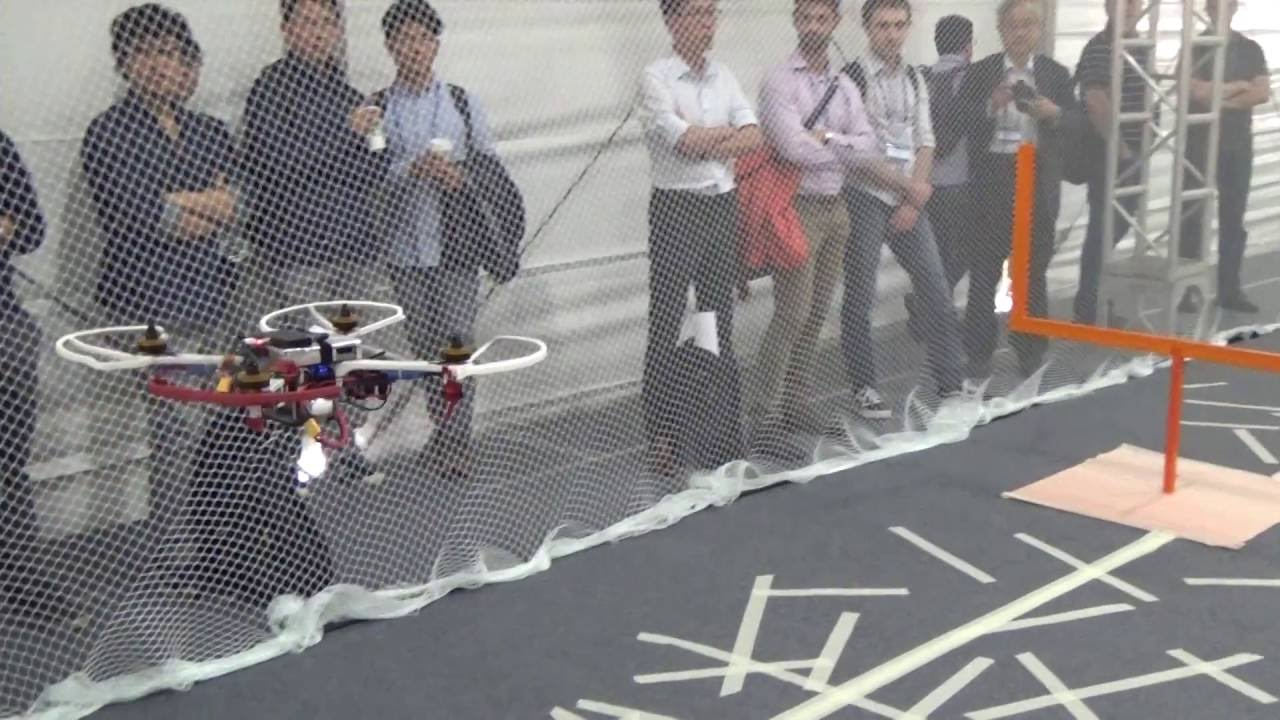
\includegraphics[width=0.5\textwidth]{figure/iros_2016.jpg}
	\caption{Drone racing arena at IROS 2016.}
	\label{fig:iros}
\end{figure}

The company Lockheed Martin is sponsoring the event and offering a prize of 2
million USD for the winning team. Teams of university students and other drone
enthusiasts shall present innovative approaches on vision-based systems for
unmanned aerial vehicles: hence, they showcase their progress through racing.\\

\section{Drone racing: definition and implications}

As in any race, competitors measure their skills at maneuvering their vehicle,
from within or at distance, against the clock or against themselves, in an
attempt to complete a circuit before everyone else.

In drone racing, the circuit consists of a set of obstacles, static or
dynamic, usually arranged in a loop. For the case of classic drone racing, huge
futuristic-looking arenas are used as a playground for extremely skilled pilots,
who make the race look impressive and dynamic by the use of FPV goggles to fly
the drones at very high speed, reaching 120mph~\cite{DRL}.

\begin{figure}[h]
	\centering
	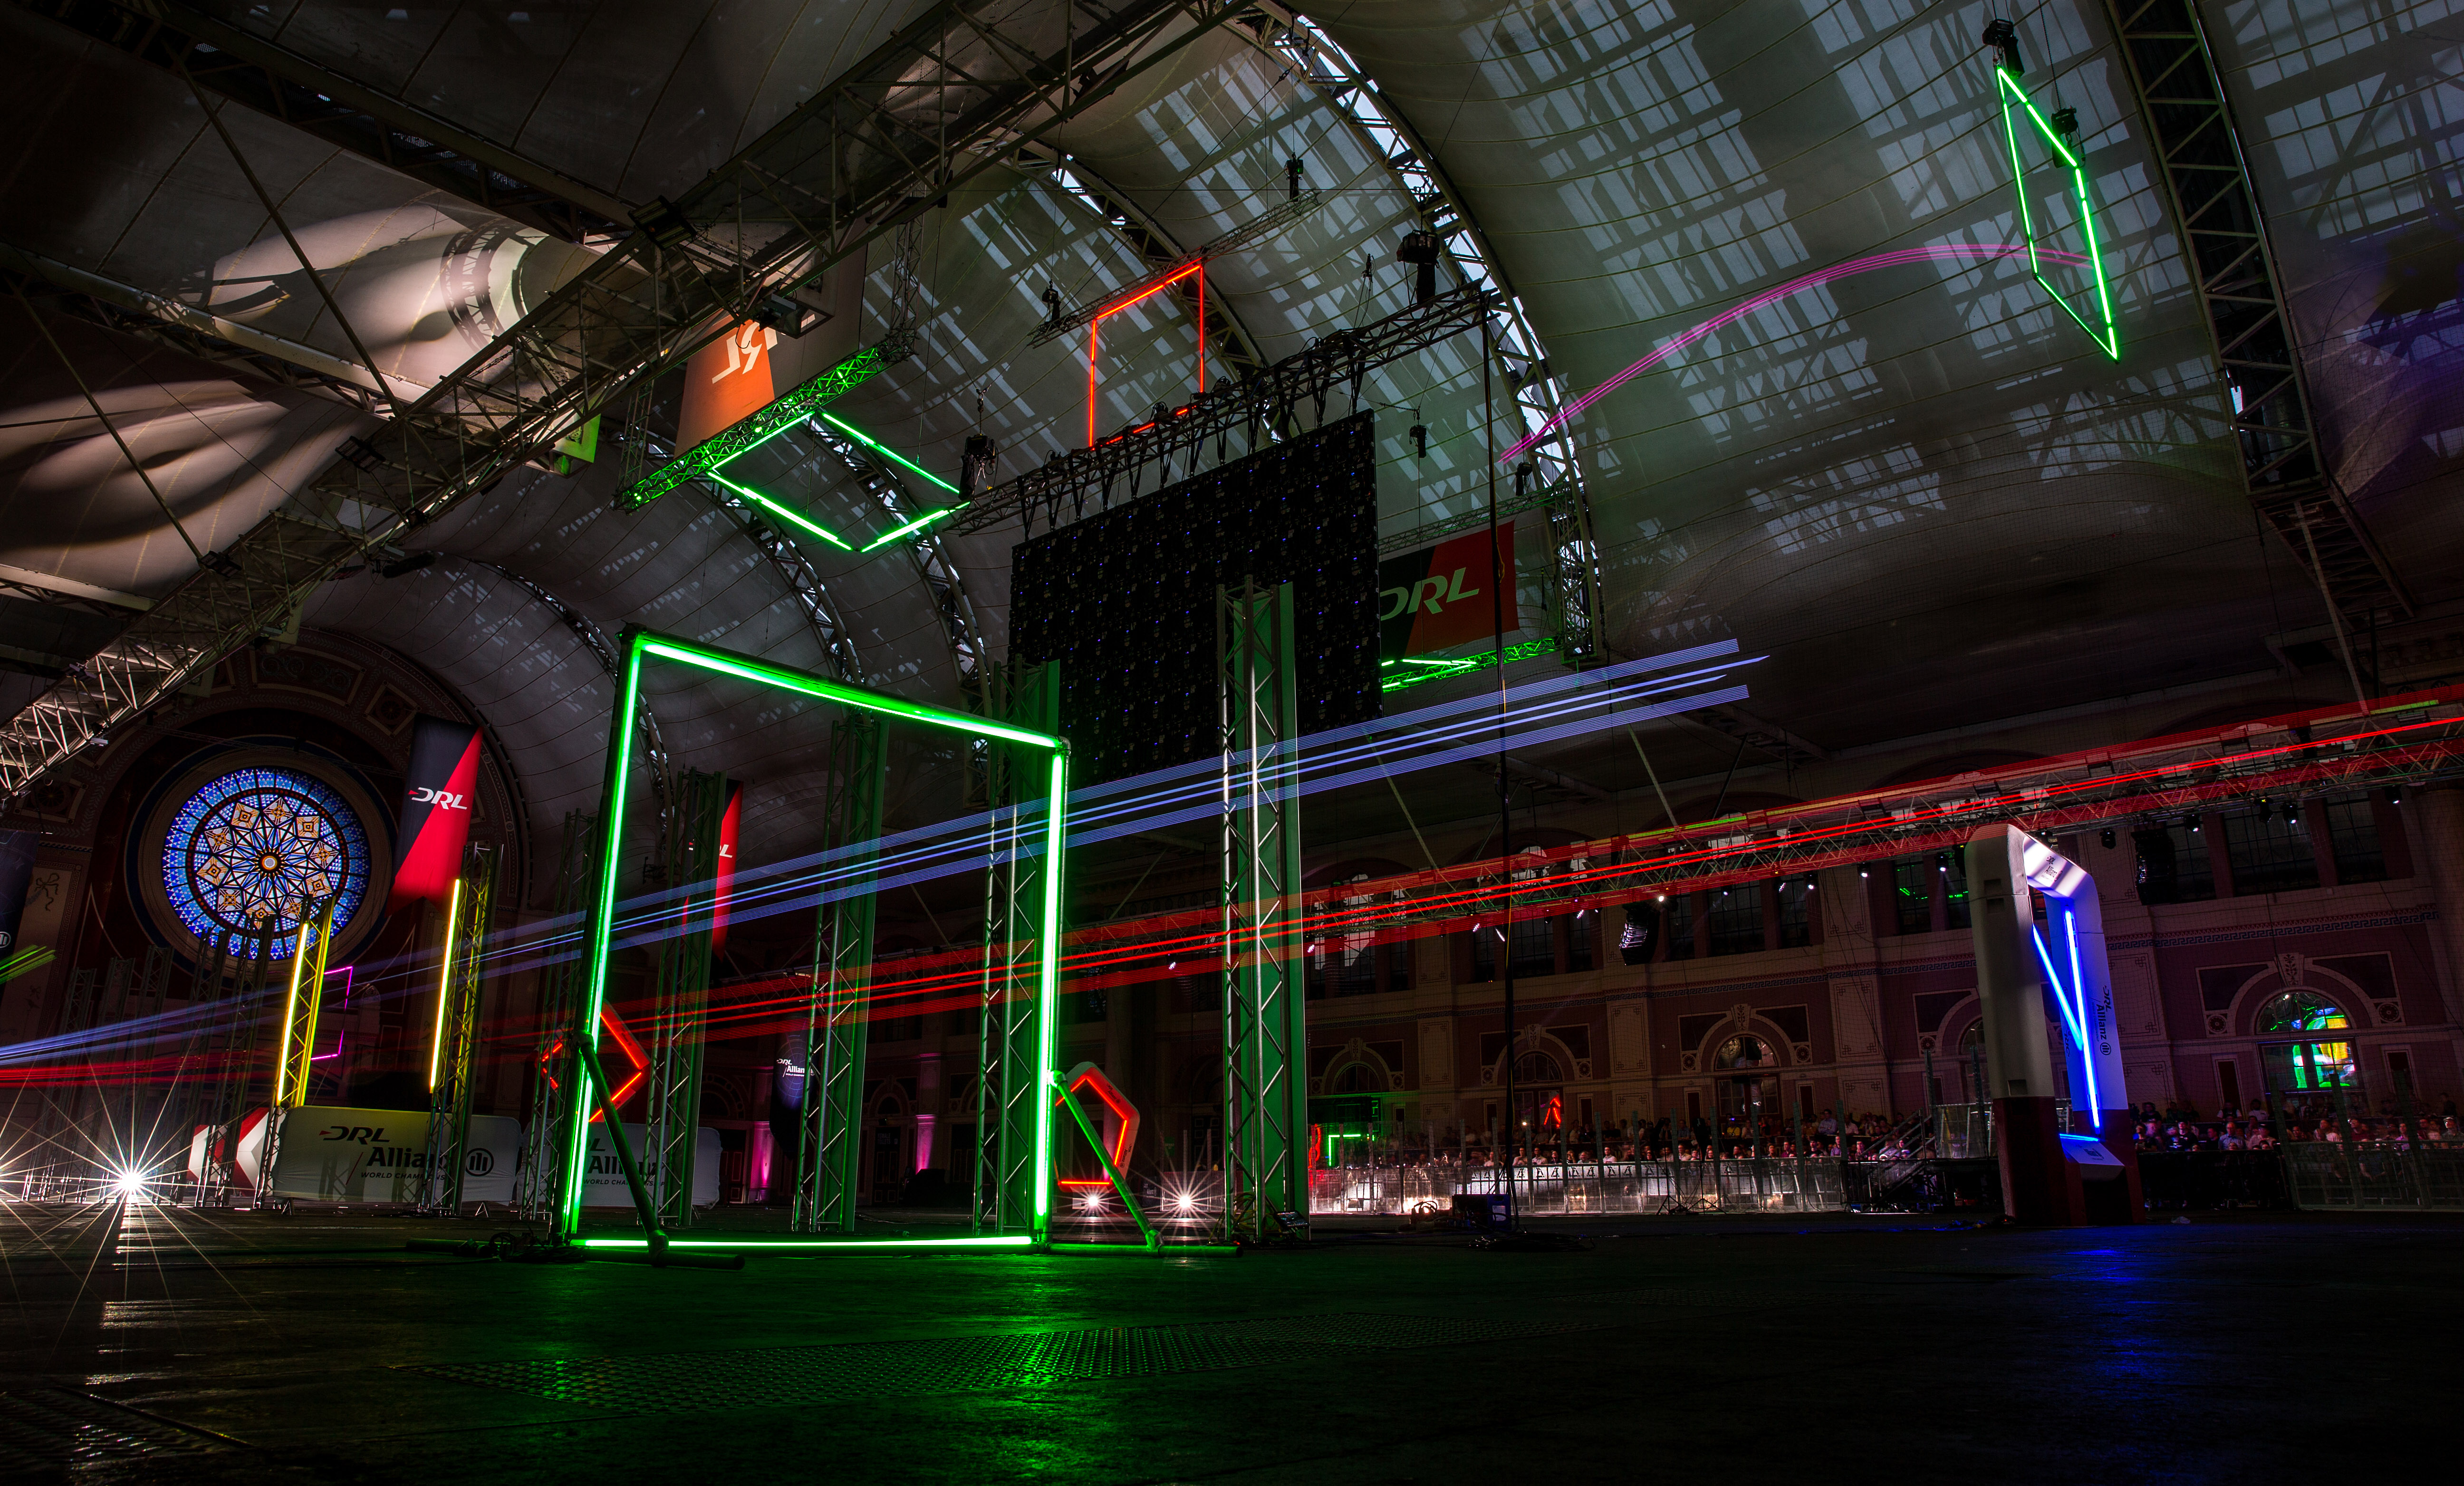
\includegraphics[width=0.5\textwidth]{figure/drl_arena.jpg}
	\caption{Drone Racing League arena in London (Steven
	Paston/PA)~\cite{DRLRecord}}
\end{figure}

For the case of autonomous drone racing, up until the \emph{Drone Racing
League} announced their autonomous competition of 2019, arenas looked much more
like a laboratory than a glowing circuit, as it can be seen on
Figure~\ref{fig:mygates} showing the AiR Lab in Skejby (Aarhus, DK), with its
gates built and painted for this work. These obstacles were inspired of the
previous competitions organized by IROS, as seen on Figure~\ref{fig:iros} which
also shows the typical type of drones used in this research area: consumer
drones for the larger audience. This kind of drones is not made for sportive
flight, but mostly for an easy hands-on experience, providing a relatively slow
but stable flight.

The goal is to complete a given amount of turns as fast as possible, but since
it is still the early days of drone racing and the costs of a potential crash
would be too high, each drone races against the clock, one after another.
Ultimately, autonomous drones will be racing against skilled pilots, as the
\emph{Drone Racing League} seems to encourage it by giving a total prize of 2
millions USD for the race of 2019~\cite{LockheedDRL}.


\begin{figure}[h]
	\centering
	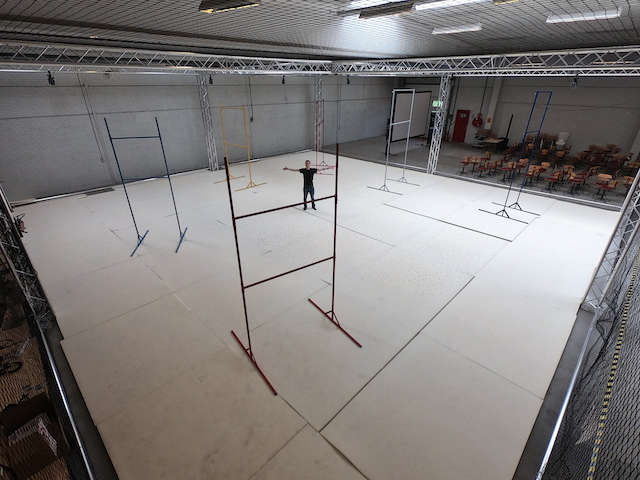
\includegraphics[width=0.5\textwidth]{figure/tiny_me.jpg}
	\caption{The AiR Lab and the custom-built obstacles around the author in Skejby}
	\label{fig:mygates}
\end{figure}

\subsubsection{Challenges}

What makes drone racing such an interesting challenge to work on for autonomous
UAVs, is the cumulative complexity of each sub-problem to be solved, namely:

\begin{itemize}
	\item{\textbf{Obstacle detection\\}
		The very first challenge to be solved is the detection of the obstacles
		on the circuit, whose shape and color can vary from competition to
		competition, and can even have dynamic properties with moving parts to
		avoid. This rather computer vision-centric problem can be solved
		in many ways, but a compromise has to be made between accuracy and
		robustness/adaptability.
	}
	\item{\textbf{Collision avoidance\\}
		In the simplest case of autonomous drone racing, the circuit is often
		composed of thin obstacles to be crossed (as seen on
		Figure~\ref{fig:mygates}), which means that the trajectory of the drone
		has little chance of encountering obstacles to avoid, if calculated
		accurately. However, it would be a valuable asset for the UAV to have
		some sort of collision avoidance system, in the case where the planned
		trajectory is wrong and the drone would crash into an obstacle, for
		instance.
	}
	\item{\textbf{Path planning\\}
		Without doubts, the most important task for an autonomous drone in the
		case of a race, is to plan its trajectory in accordance with its
		surroundings. An efficient trajectory must be as direct as possible,
		from point A to B, where B is usually a gate through which the drone
		has to pass, or even the end point of the race (in which case the
		trajectory must also go through every gate).
	}
	\item{\textbf{Circuit compliance\\}
		Being able to generate an efficient trajectory is already an
		achievement, but it is to no use in a race if it is not respecting the
		order of the obstacles which the drone must fly through. In some cases,
		a rough map of the circuit is given a short time before the
		competition, so that participants can take the desired trajectory in
		consideration when developing their algorithm.
	}
	\item{\textbf{Aggressive flight\\}
		Last but not least, any pilot, being human or software, must be able to
		drive fast and aggressively in order to have a chance of winning a
		race.  Nevertheless, this is a challenge on its own that does not need
		to be solved until every building block of the auto-pilot system is
		robust and efficient.\\
	}
\end{itemize}

This list is only a gross summary of the main challenges of autonomous drone
racing, and only scratches the surface of all the issues that must be
considered. One core piece of logic in autonomous drone racing is the decision
making. This is an entire topic on its own, and it is applied to many other
areas, ranging from finance to artificial intelligence. In the case of
autonomous drone racing, decisions have to be made constantly with regards to
crossing gates, avoiding obstacles, or maintaining a course. A chapter is
dedicated to this subject, further in this report.

The following section delves deeper into the specific problems that are solved
in this thesis, after an analysis of the state of the art and the methods
commonly used to solve those problems.



\section{Literature review}

\todo{Insert literature review as a table}

\subsection{The modern approach}
As it can be seen from the preceding literature review, most robotic systems'
operation can be modeled by the commonly known \emph{Sense, Plan, Act}
paradigm:

\todo{Add custom act, sense, plan paradigm picture}
\begin{figure}[h]
	\centering
	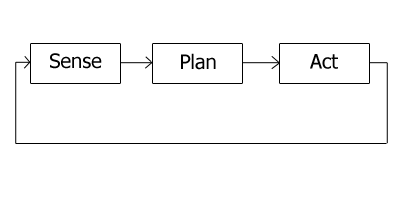
\includegraphics[width=0.4\textwidth]{figure/robotic_paradigm.png}
	\caption{The Sense, Plan, Act robotic paradigm. [temp, will make my own]}
	\label{fig:robotic_paradigm}
\end{figure}

\begin{itemize}
	\item{\textbf{Sense}}: gather information using sensors (camera, IMU, sonar...).
	\item{\textbf{Plan}}: create a world model using all the information, and plan
		the next move.
	\item{\textbf{Act}}: carry out the actions that the plan calls for.
\end{itemize}

~\\
This thesis will be focused mainly on the sensing of the drone control, and
more precisely using deep learning and computer graphics. However, an important
part of the trajectory planning directly follows the sensing phase, therefore
those two first phases of the control loop can be included in the scope of the
project.

To this day, most drones in the robotic research field are running \emph{Robot
Operating System} (ROS), \todo{Add citation} which is a set of ``libraries and
tools to help software developers create robot applications''. It allows to
independently run programs as ``nodes'', which can communicate with each other
using a principle of ``subscription'' and ``publication`` on easily definable
topics, as represented on Figure~\ref{fig:ros-topics}.

\begin{figure}[h]
	\centering
	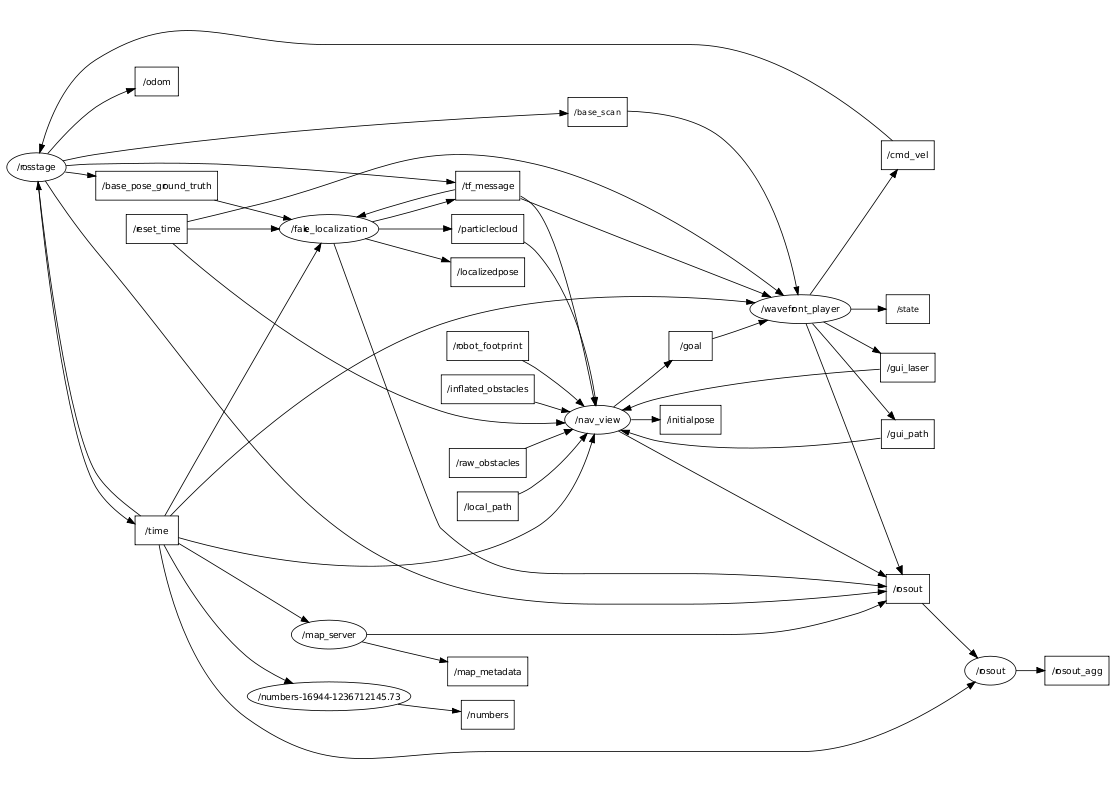
\includegraphics[width=0.7\textwidth]{figure/ros_topics.png}
	\caption{The ROS topics graph showing inter-node communications for this
	project. [temp, will make my own]}
	\label{fig:ros-topics}
\end{figure}

ROS makes the transition between the simulated environment and the real world
seamless, because it can be installed on most Linux systems, and adds a layer
of abstraction between the hardware and the software, by distributing packages
built by the community.\\

The implementation of the computer vision algorithms will be constrained within
ROS, and cooperate with the different control components, in an effective
modular manner.\\

\todo{Talk about why CNNs are used more and more in drone racing, and basically
why it is the chosen approach, which leads to tackling the dataset generation
problem.}


As deep learning has known an exponential growth during the past decade,
computer vision applications tend to exploit the power of convolutional neural
networks more and more. Thanks to their impressive performance in specific
problem solving, CNNs are becoming the main choice for tasks such as: object
detection, object segmentation, object recognition, object tracking,
\emph{etc}\ldots

In drone racing, the latest works, which are often the best performing, tend to
employ CNNs for the sensing part, or even as an all-in-one solution. It is a
reasonable choice mainly because neural networks are observed to offer
robustness and accuracy, to the cost of computational power. They can be hard
to train, given their sporadic nature, but it is often a very good alternative
to developing a custom algorithm which can take a lot of time and does not
guarantee consistent results, in different lighting conditions for instance.

On that note, the chosen method for solving the drone racing challenge is
using a convolutional neural network, coupled with a simple state-machine 
using a PID controller to steer the drone.


\section{Proposed approach}

In order to make things easier and to be able to set tangible milestones, the
challenge is split in two logical problems to be solved, one after the
other, namely:
\begin{enumerate}
	\item{\textbf{Gate center detection:\\}
			The geometric center of the nearest gate in the field of view of the
			drone is to be recognized in real time.
	}
	\item{\textbf{Trajectory planning:\\}
			A trajectory between the current drone position, and the targeted gate
			center is to be generated in real time.
	}
\end{enumerate}

\begin{figure}[h!]
	\centering
	\begin{tikzpicture}[node distance=2cm,-latex]

\pgfdeclarelayer{background}
\pgfdeclarelayer{foreground}
\pgfsetlayers{background,main,foreground}
\tikzstyle{sensor}=[node distance=1.5cm,draw, rectangle,fill=blue!20, text width=2cm,text centered,minimum width=2cm, minimum height=1cm]
\tikzstyle{perc}=[draw, node distance=4cm,draw, rectangle,fill=green!20, text width=2cm,text centered,minimum width=2cm, minimum height=1cm]
\tikzstyle{control}=[draw, node distance=3cm,draw, rectangle,fill=red!20, text width=2cm,text centered,minimum width=2cm, minimum height=3cm]

%% Sensors Nodes 
\node[sensor] (cam) {Camera};
\node[sensor,below of=cam] (imu) {IMU};
\node[sensor,below of=imu] (lidar) {Lidar};
\node[node distance=1cm,above= of cam.west,anchor=west] (sensors) {Sensors};

\begin{pgfonlayer}{background}
    \node[fit=(sensors) (cam) (imu) (lidar), draw,fill=yellow!20] (frame) {}; 
\end{pgfonlayer}

%% Perception Nodes
\node[perc,node distance=4cm,right of=cam] (cnn) {CNN};
\node[perc,right of=cnn] (median) {Median Filter};
\node[node distance=1cm,above= of cnn.west,anchor=west] (perception) {Perception};

\begin{pgfonlayer}{background}
    \node[fit=(perception) (cnn) (median), draw,fill=yellow!20] (frame) {}; 
\end{pgfonlayer}

%% Control Nodes
\node[control,node distance=4.5cm,below of=cnn] (state) {State Machine};
\node[control,right of=state,minimum width=2cm,minimum height=1cm,yshift=1cm] (pid) {PID};
\node[control,right of=pid,minimum width=2cm,minimum height=1cm] (safety) {Safety Mechanism};
\node[control, node distance=2cm,below of=safety,minimum width=4cm,minimum height=1cm] (low) {Low Level Control};
\node[node distance=2cm,above= of state.west,anchor=west] (controller) {Control};

\begin{pgfonlayer}{background}
    \node[fit=(state) (pid) (safety) (low) (controller), draw,fill=yellow!20] (frame) {}; 
\end{pgfonlayer}

%% Connections
\draw[thick] (cam) -- (cnn);
\draw[thick] (cnn) -- (median);
\draw[thick] (lidar.east) -- ++(1cm,0) |- (state);
\draw[thick] (imu) -| ($(pid.north west)!0.33!(pid.north east)$);
\draw[thick] (pid.west) -- ($(state.north east)!0.17!(state.south east)$);
\draw[thick] ($(state.north east)!0.5!(state.south east)$) -| ($(safety.south west)!0.33!(safety.south east)+(0,-0.5cm)$) -- ($(safety.south west)!0.33!(safety.south east)$);
\draw[thick] (pid) -- (safety);
\draw[thick] ($(safety.south west)!0.66!(safety.south east)$) --  ($(low.north west)!0.59!(low.north east)$);
\draw[thick] (median) -- ++(0,-1.5cm) -|($(pid.north west)!0.66!(pid.north east)$);

\end{tikzpicture}

	\caption{Block diagram of the system.}
	\label{fig:block-system}
\end{figure}

~\\The problem is not solved as a whole race, but rather as a trajectory
between a starting point and a gate. This choice of approach is motivated by
the fact that admittedly, if the nearest gate detection is quick and precise,
considering a race as a succession of independent targets to be reached is
theoretically a robust solution that can be applied to any environment, with any
obstacles, and of any length.\\

Firstly, the perception logic is solved with a deep learning algorithm, most
precisely a convolutional neural network. However, it has been seen from
the literature review that collecting a dataset for drone racing can be
tedious, and is rarely variate enough to allow for good generalization of the
learning and application in any given environment. In this work, a
semi-synthetic dataset is generated from background images, to provide an
infinite amount of circuit combinations to train the gate recognition network
(more on that in the following chapter).

In order to detect the closest gate's center, which is the point where the
drone will have to fly through, the problem is simplified so that the output of
the CNN can be directly used by the control logic, without any processing,
except filtering. As shown on figure~\ref{fig:regionproposal}, the input image
is treated as a grid of $N$ windows, numbered from $1$ to $N$ and left to
right, where the closest gate's center is either inside, or outside. The reason
for the indexing to start at $1$ is justified by the presence of a ``virtual''
window, numbered $0$, which represents the absence of any gate center in the
image. In total, $N+1$ region proposal windows are considered for the gate
center detection algorithm, event though only $N$ windows actually split the
image in a grid.

\begin{figure}[h!]
	\center
	\includegraphics[width=0.7\textwidth]{figure/region_proposal.png}
	\caption[Visual representation of the region proposal grid]{A visual
		representation of the region proposal for the closest gate's center, with
		$N=25$, where the ground truth is annotated in red (window 17), and the gate
		center as the green cross.}
	\label{fig:regionproposal}
\end{figure}

The amount of windows -- minus window $n^{\circ}0$, thus $N$ -- for the region
proposal of the closest gate's center can be adjusted for a more precise
trajectory, but must be a perfect square number to work with the current
implementation, as it greatly simplifies the computation of the ground truth
labels.

Finally, a median filter is applied to the predictions, in order to remove the
outliers. This addition aims to prevent the drone from deviating from the
optimal path, even though a small delay is introduced in the perception.

Being the main research topic of this thesis, this part is given more time and
focus to deliver a more rigorous and in-depth work.\\

%\begin{figure}[h]
	%\centering
	%
\includegraphics[width=0.5\textwidth]{figure/300x300.png}
	%\caption{Block diagram of the perception logic.}
	%\label{fig:perception-block}
%\end{figure}

Secondly, the control logic is made as simple as can be, since its purpose is
only to verify the hypothesis proposed for the perception. A state machine is
supervising the flight between the two gates, and utilizes a
Proportional-Integral-Derivative controller to output velocity commands to the
lower-level controller implemented by the manufacturer on the UAV.\\

%\begin{figure}[h]
	%\centering
	%
\includegraphics[width=0.5\textwidth]{figure/300x300.png}
	%\caption{Block diagram of the control logic.}
	%\label{fig:control-block}
%\end{figure}

As for the drone itself, the model used to conduct real flight tests is an Intel
Aero, a customizable platform built for developers. It is ready to fly, and
comprises several sensors, namely:

\begin{itemize}
	\item{Intel Atom® x7-Z8750 processor}
	\item{4 GB LPDDR3-1600}
	\item{32 GB eMMC}
	\item{Intel® RealSense™ R200 camera}
		\begin{itemize}
			\item{Depth/infrared: 640x480 resolution at 60FPS}
			\item{RGB: 1080p at 30FPS}
		\end{itemize}
	\item{OmniVision OV8858 8MP RGB camera (front facing)}
		\begin{itemize}
			\item{3264x2448 at 30FPS}
			\item{1080p at 60FPS}
			\item{720p at 90FPS}
			\item{Electronic Image Stabilization}
		\end{itemize}
	\item{OmniVision OV7251 VGA camera, global shutter, monochrome (down facing)}
	\item{GPS and compass}
	\item{Intel® Aero Flight Controller with Dronecode PX4 Autopilot}
\end{itemize}

~\\Since it comes with the Yocto Project~\cite{Yocto} Linux distribution
pre-installed, Ubuntu 16.04 had to be setup first before installing ROS
Kinetic. Unfortunately, the OmniVision OV8858 front facing camera is not
supported on Linux distributions other than the Yocto Project, which means its
high speed video recording feature couldn't be taken advantage of to eliminate
as much motion blur as possible, and instead, the RealSense™ R200 camera is
used. Having a high resolution would be of no interest, since it would only
make the CNN run slower in despite of a negligible gain in accuracy.\\


The solution will be implemented iteratively, by gradually increasing the
complexity of the vision algorithms, such that progress can be made even if the
end goal is too difficult to achieve.\\

The project should attempt to fulfill the following goals:

\begin{itemize}
	\item{Recognize gates in the input image}
	\item{Detect and localize the closest gate's center}
	\item{Evaluate the closest gate's orientation and distance}
	\item{Plan a trajectory for the drone to fly across the gate center}
	\item{Refine the trajectory in real time, for an optimal flight time}
	\item{Make the drone follow that trajectory while adjusting in real time}
\end{itemize}
~\\
However, the following functionalities are out of the scope and will be
discarded:

\begin{itemize}
	\item{Detect any other obstacles in the input image}
	\item{Avoid obstacles that are on the drone's trajectory}
	\item{Map and localize the detected gates in world frame}
	\item{Plan a trajectory of a sequence of gates}
	\item{Apply online learning for adaptive racing}
\end{itemize}

